\documentclass[12pt,twoside]{report}

\author{Oliver Kohlbacher}
\title{
	\begin{center}
		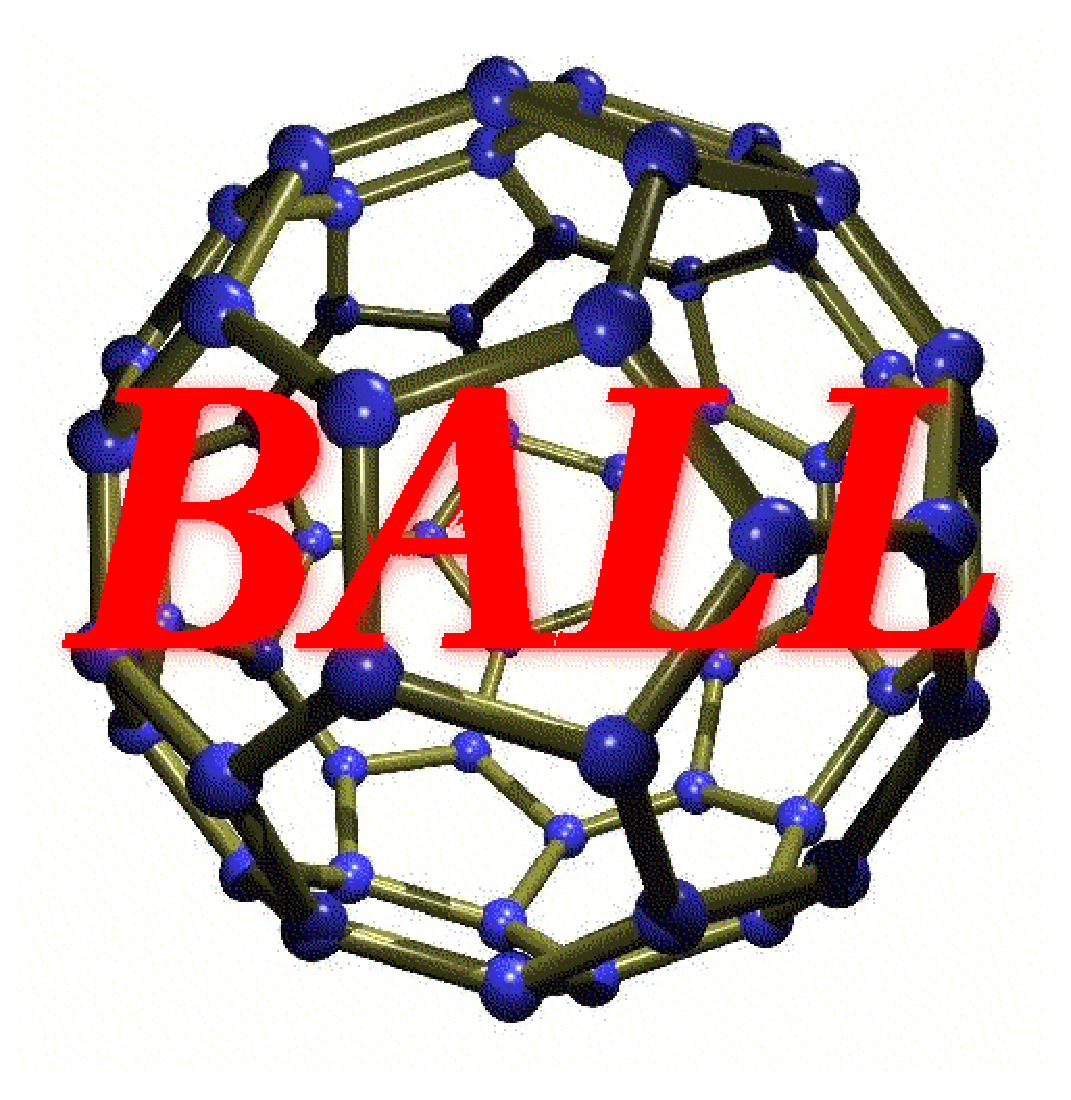
\includegraphics[width=10cm]{logo.eps}
	\end{center}
	\Huge How to BALL\\ 
	\Large A Tutorial
}

%-----------------------------------------
% used packages
%-----------------------------------------
\usepackage{a4}
% use A4 paper

%\usepackage[draft]{graphicx}
\usepackage{graphicx}
% use graphics pacakge

\usepackage{times}
% use postscript fonts

\usepackage{psboxit}
\newcommand{\graybox}[1]{\psboxit{box .85 setgray fill}{\fbox{#1}}}
% display gray shaded boxes using postscript commands
%


%-----------------------------------------
% quote environment for quatations
%-----------------------------------------
% in part stolen from LaTeX companion
\usepackage{ifthen}
\newsavebox{\QuoteNameBox}
\newenvironment{Quote}[1]%
	{%
		\sbox{\QuoteNameBox}{{\it #1}}%
		\begin{list}{}{%
			\setlength{\rightmargin}{\leftmargin}}%
				\item[]``\ignorespaces}%
	{\unskip''\hfill \usebox{\QuoteNameBox}\end{list}}


\usepackage{changebar}
% This package defines the two commands \cbstart and \cbend. It then displays a
% bar between the start and the end command

\usepackage{color}
% This package allows the coloring of text (e.g. in an ipe minipage)

\usepackage{float}
% the float package allows a better placement of all floats (figures,tables) or
% even new floats it allows the following kinds of boxes:
% \shadowbox, \doublebox, \ovalbox, \Ovalbox

\makeatletter
	\renewcommand{\@makecaption}[2]{
		\vspace{3pt}
		\noindent{\color{blue}\rule{\textwidth}{1pt}}\par
		\noindent{\small{\sffamily #1:}\hspace{5pt}\itshape #2\par}
		\vspace{5pt}
	}
\makeatother
% 
%  create a fancy float caption: 
%    - blue rule under the float
%    - the figure text set in sans serif
%    - the caption text in italics

\setcounter{topnumber}{1}
\setcounter{bottomnumber}{1}
%
%  	some settings for the floats: just on float at the
%		top of a page and on at the bottom

	
%-----------------------------------------
% Font definitions 
%-----------------------------------------

\usepackage{amsfonts}
\usepackage{amsmath}
\usepackage{amsthm}
\usepackage{amssymb}

%-----------------------------------------
% Textlayout 
%-----------------------------------------

\newcommand{\clearemptydoublepage}{\newpage{\pagestyle{empty}\cleardoublepage}}

%\usepackage{a4wide}
\setlength{\textheight}{21cm}
\setlength{\textwidth}{14.5cm}
\setlength{\oddsidemargin}{10mm}
\setlength{\evensidemargin}{2mm}
\setlength{\topmargin}{0mm}
%\setlength{\marginparsep}{5mm}
%\setlength{\marginparwidth}{2cm}
%\renewcommand{\baselinestretch}{1.21}
\large\normalsize

%-----------------------------------------
% some shorthands
%-----------------------------------------

\providecommand{\R}{\mathbb R}
\providecommand{\Q}{\mathbb Q}
\providecommand{\N}{\mathbb N}
\providecommand{\Z}{\mathbb Z}

%-----------------------------------------
% redefinitions of sectioning comands
%-----------------------------------------

\usepackage{fancyheadings}
% allows you an easy adaption of the headings

\usepackage{fancybox}
% you can use shaded boxes e.g. for figures it allows the following kinds of boxes:
% \shadowbox, \doublebox, \ovalbox, \Ovalbox

\addtolength{\headrulewidth}{0.2pt}
\addtolength{\footrulewidth}{0.6pt}
\addtolength{\headwidth}{1cm}
\addtolength{\footskip}{10mm}
\addtolength{\headsep}{5mm}
\addtocounter{secnumdepth}{2}
\setcounter{tocdepth}{3}
\setcounter{secnumdepth}{3}

\renewcommand{\chaptermark}[1]{\hfill\markboth{#1}{}\hfill}
\renewcommand{\sectionmark}[1]{\hfill\markright{\thesection\ #1}\hfill}
\lhead{}
\rhead{}
\chead[\fancyplain{}{\textrm{\leftmark}}]%
      {\fancyplain{}{\textrm{\rightmark}}}
\cfoot{}
\rfoot[\fancyplain{}{}]{\fancyplain{}{\bfseries\thepage}}
\lfoot[\fancyplain{}{\bfseries\thepage}]{\fancyplain{}{}}


% the \chapter ...
\makeatletter
%\renewcommand\thesection 			{{\sffamily\thechapter.\@arabic\c@section}}
%\renewcommand\thesubsection   {{\sffamily\thesection.\@arabic\c@subsection}}
%\renewcommand\thesubsubsection{{\sffamily\thesubsection.\@arabic\c@subsubsection}}
\renewcommand{\@chapapp}{\sffamily}
%\renewcommand\section{\@startsection {section}{1}{\z@}%
%	{-3.5ex \@plus -1ex \@minus -.2ex}%
%	{2.3ex\@plus.2ex}%
%	{\normalfont\Large\sffamily\bfseries}
%}
%\renewcommand\subsection{\@startsection{subsection}{2}{\z@}%
%	{-3.25ex\@plus-1ex \@minus -.2ex}%
%	{1.5ex \@plus .2ex}%
%	{\normalfont\large\sffamily\bfseries}
%}
%\renewcommand\subsubsection{\@startsection{subsubsection}{3}{\z@}%
%	{-3.25ex\@plus-1ex \@minus -.2ex}%
%	{1.5ex \@plus .2ex}%
%	{\normalfont\normalsize\sffamily\bfseries}
%}
\makeatother

%-----------------------------------------
% macro for missing pieces
%-----------------------------------------
\usepackage{changebar}
\newcommand{\missing}[1]{
	\cbstart  % add a gray bar at the side of the page
	\message{^^JMISSING: #1^^J}
	\par\noindent\fbox{{\bf MISSING:} #1}\par
	\cbend
}

%-----------------------------------------
% rules for figures
%-----------------------------------------

\topfigrule
\botfigrule
\setlength{\shadowsize}{2pt}

%-----------------------------------------
% some shorthands
%-----------------------------------------

\usepackage{xspace}
% you should use \xspace in defining shorthands 
% e.g. \newcommand{\eg}{e.g., \xspace} \@ is for the correct spacing after punctuation

\newcommand{\eg}{{\it e.g.}\xspace}
\newcommand{\ie}{{\it i.e.}\xspace}
\newcommand{\ea}{{\it et al.}\xspace}
\newcommand{\etc}{{\it etc.}\xspace}
\def\CPP{C\raise.08ex\hbox{\tt ++}\xspace}


%-----------------------------------------
% the index
%-----------------------------------------
\usepackage{makeidx}

\newcommand{\Index}[1]{#1\index{#1}}
% prints the term and creates an index entry

\newcommand{\class}[1]{{\ttfamily{#1}}\index{#1@{\ttfamily{#1}}
(BALL~class)}\index{BALL!classes!#1@{\ttfamily{#1}}}}
% BALL class names are typeset in typewriter bold and indexed automatically:
%  - first with their class name
%  - then under BALL!classes!<classname>

\newcommand{\STLclass}[1]{{\ttfamily{#1}}\index{#1@{\ttfamily{#1}}
(STL~class)}\index{STL!#1 class@{\ttfamily{#1}}}}
% STL class names are typeset in typewriter bold and indexed automatically:
%  - first with their class name
%  - then under STL!<classname> class

\newcommand{\function}[1]{{\ttfamily{#1}}\index{#1@{\ttfamily{#1}}
(BALL~function)}\index{BALL!functions!#1@{\ttfamily{#1}}}}
% BALL function names are typeset in typewriter bold and indexed automatically:
%  - first with their name
%  - then under BALL!functions!<function name>

\newcommand{\method}[1]{{\ttfamily{#1}}\index{#1@{\ttfamily{#1}}
(method)}\index{BALL!functions!#1@{\ttfamily{#1}}}}
% method names are typeset in typewriter bold and indexed automatically:
%  - first with their name
%  - then under BALL!methods!<function name>

\newcommand{\attribute}[2]{{\ttfamily{#1}}\index{#1@{\ttfamily{#2}}
({\ttfamily #1} attribute)}\index{BALL!!#1!#2@{\ttfamily{#1}}}}
% attribute names are typeset in typewriter bold and indexed automatically:
%  - first with their name and (<class> attribute)
%  - then under BALL!<class>!<attribute>

\newcommand{\macro}[1]{{\ttfamily{#1}}\index{#1@{\ttfamily{#1}}
(BALL~macro)}\index{BALL!macros!#1@{\ttfamily{#1}}}}
% BALL macros names are typeset in typewriter bold and indexed automatically:
%  - first with their name
%  - then under BALL!macros!<macro name>

\newcommand{\namespace}[1]{{\ttfamily{#1}}\index{#1@{\ttfamily{#1}}
(BALL~namespace)}\index{BALL!namespaces!#1@{\ttfamily{#1}}}}
% BALL macros names are typeset in typewriter bold and indexed automatically:
%  - first with their name
%  - then under BALL!namespaces!<name>

\newcommand{\type}[1]{{\ttfamily{#1}}\index{#1@{\ttfamily{#1}}
(BALL~type)}\index{BALL!types!#1@{\ttfamily{#1}}}}
% BALL macros names are typeset in typewriter bold and indexed automatically:
%  - first with their name
%  - then under BALL!types!<macro name>

\newcommand{\file}[1]{
	{\ttfamily\mbox{#1}}
	\index{#1@{\ttfamily{#1}} (file)}
}
% BALL file names are typeset in typewriter bold and indexed automatically:
% with their name and "(file)" appended

\newcommand{\directory}[1]{
	{\ttfamily\mbox{#1}}
	\index{#1@{\ttfamily{#1}} (directory)}
}
% BALL directories are typeset in typewriter bold and indexed automatically:
% with their name and "(directory)" appended

\newcommand{\option}[1]{
	{\ttfamily\mbox{#1}}
	\index{configure!options!#1@{\ttfamily\mbox{#1}}}
}
% BALL file names are typeset in typewriter bold and indexed automatically:
% as configure/options/<name>"

\newcommand{\exception}[1]{{\ttfamily{#1}}\index{#1@{\ttfamily{#1}}
(BALL~class)}\index{BALL!exceptions!#1@{\ttfamily{#1}}}}
% BALL exceptions names are typeset in typewriter bold and indexed automatically:
%  - first with their name
%  - then under BALL!exceptions!<exception name>

\newcommand{\newtermdef}[1]{{\em #1}\index{#1!definition}}
% prints the term in italics and includes creates an index entry
% with the subentry "definition"

\newcommand{\newterm}[1]{{\em #1}\index{#1}}
% prints the term in italics and creates an index entry

\newcommand{\URL}[1]{{\bfseries\ttfamily\mbox{#1}}}
\newcommand{\email}[1]{{\bfseries\ttfamily\mbox{#1}}}

%--------------------------------------------
%  the style of embedded listings
%--------------------------------------------
\usepackage{listings}
% formatting of the listings
\lstset{
	%% we use ANSI C++
	language=[ANSI]C++,
%
	%% our tabs are always expanded to 2 blanks
	tabsize=2,
%
	%% the font size of the listing
	basicstyle=\small\ttfamily,
%
	%% make the listing as wide as \textwidth
	spread=-0.3cm,
%
	%% draw a line at the left of the listing
	frame=tlrb,
%
	%% captions appear at the bottom of the listing
	%captionpos=b,
%
	%% and make the corners of the frame round
	frameround=tttt,
%
	%% the label font
	labelstyle=\sffamily,
%
	%% line numbers for each line
	labelstep=0
}
\newcommand{\linelisting}{\lstinline[frame=,basicstyle=\small]}


%%
%%
%%     FAQ macros
%%
\newcounter{FAQcounter}
\setcounter{FAQcounter}{0}
\newcommand{\FAQquestion}[1]{%
	\ifthenelse{\theFAQcounter=0}{}{\vspace{0.5cm}\begin{center}\rule{0.5\textwidth}{1pt}\end{center}\vspace{0.5cm}}%
	\stepcounter{FAQcounter}%
	\noindent{\bf Question \theFAQcounter:} {\em #1 \par}%
}
\newcommand{\FAQanswer}[1]{\bigskip\noindent{\bf Answer:} #1\par}	
\newcommand{\FAQURL}[1]{{\tt #1}}

\pagestyle{fancyplain}
\sloppy
\makeindex

\begin{document}
\maketitle

\pagenumbering{roman}
\setcounter{page}{1}
\tableofcontents
\pagenumbering{arabic}
\setcounter{page}{1}

\chapter{Introduction}
\label{chapter:introduction}
\noindent
BALL (Biochemical Algorithms Library) is an application framework for rapid
software prototyping in the field of Molecular Modeling.  This tutorial shall
help new users to make their first steps with BALL. It is {\em not} a full
documentation. For a full documentation, please refer to the \newterm{Reference
Manual}~\cite{BALL-RM} which can be obtained in HTML, PDF, or postscript format.

There are also several papers and technical reports published on
BALL~\cite{BKL99a,BKL99b,KL99,Koh2001,KL2000,MHLK05,MHLK06}
that give a cursory overview of its design principles and illustrate its use in
Rapid Software Prototyping. If you publish results that were obtained using 
BALL, please cite it as follows:
\begin{enumerate}
  \item[] O. Kohlbacher, H.-P. Lenhof: BALL -- Rapid Software Prototyping
          in Computational Molecular Biology, {\em Bioinformatics} 2000,
          16(9):815--824
\end{enumerate}

\noindent
The latest version of BALL, bug fixes, and updates are available from our 
website

\begin{enumerate}
  \item[] \URL{http://www.ball-project.org}
\end{enumerate}

\noindent 
as well as further documentation, bug reports, and changes.

The next section of this tutorial gives a short overview of the structure and
contents of BALL. Chapter \ref{chapter:getting-started} describes the
installation and related issues. In Chapter \ref{chapter:first-steps}, some
fundamental concepts and classes are explained. After that we will show how to
use more advanced features of BALL. We will have a general overview of BALL 
 (Chapters \ref{chapter:foundation-classes} and  \ref{chapter:kernel}) 
and the usage of the visualization parts of BALL (Chapter \ref{chapter:view-programming}). 
Chapter \ref{chapter:python} will show you
the mechanisms and the usage of BALL's Python bindings.  Finally, Chapter
\ref{chapter:faq} tries to answer some of the most frequently asked questions.

\section{Overview}
\index{BALL!overview}

The basis of all BALL classes is an extensive set of \newterm{foundation
classes}.  They provide generic implementations of advanced data structures
(\eg, trees, hash associative containers, hash grids, \etc), mathematical
objects (\eg, matrices, vectors, geometric objects), implementations of
\Index{design patterns}, object \Index{persistence}, and access to the
operating system (\eg, networking support, file handling). An overview of the
overall structure of BALL is given in Fig. \ref{fig:BALL_structure}.

The BALL \newterm{kernel} contains the molecular data structures for the
representation of atoms, bonds, molecules, proteins, \etc  The kernel classes
are implemented with the foundation classes and are carefully designed to
provide maximum extensibility and flexibility.
\begin{figure}[tb]
  \centering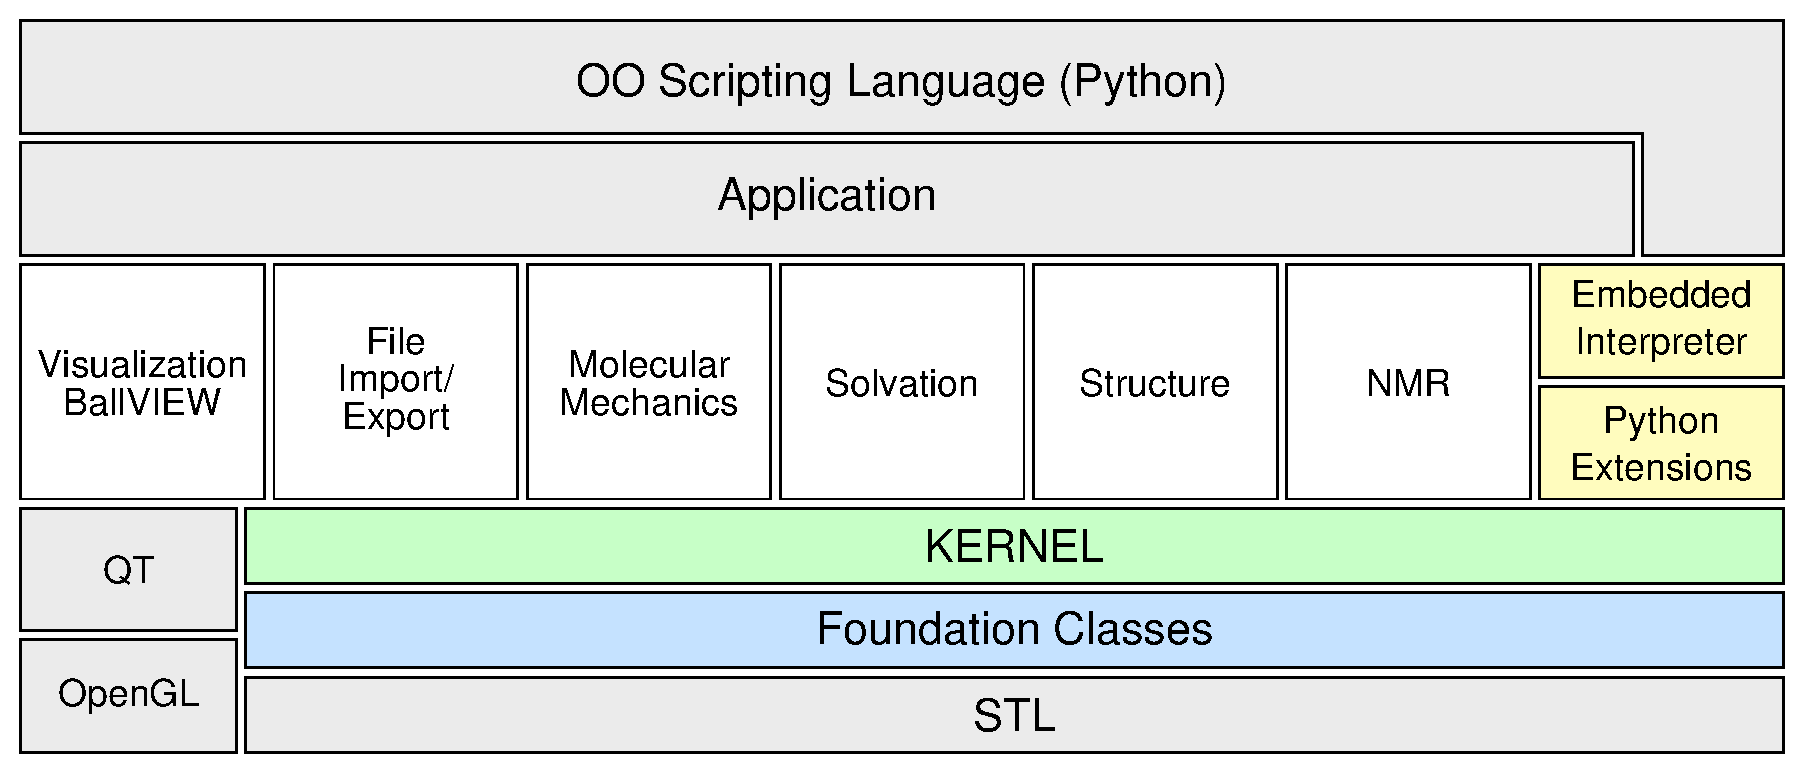
\includegraphics[width=\textwidth]{BALL_structure.eps}
  \caption{Overview of the structure of BALL}
  \label{fig:BALL_structure}
\end{figure}

The third layer of classes (on top of the foundation classes and the kernel)
provides the functionality required for applications. We call them
\newterm{basic components}. Each of these basic components is independent of
the other components.  We have implemented five basic components that cover
\Index{Molecular Mechanics}, file import/export, advanced \Index{solvation
methods}, structure analysis/comparison and \Index{visualization}. These
areas were selected, because our main interest stems from the field of protein
docking. The Molecular Mechanics component does not only provide standard
force fields (AMBER~\cite{AMBER95}, CHARMM~\cite{BBO+83}), but also a generic
\Index{force field}.  This generic force field is a base class for all force
fields. It implements fundamental methods to manage parameter files, parameter
assignment, and atom type assignment, and defines a common interface for all
force fields. Thus, large portions of code may be reused for the
implementation of new force fields.  The file import/export component
implements general methods for efficient file handling, but also methods to
read and write the most common file formats used for molecular structures
(\eg, PDB, MOL2). The solvation component provides methods for calculating
solvation effects. The first method that accounts for solvation is the atomic
contact energy by Zhang {\it et al.}~\cite{ZVC+97}. The second approach that
we implemented is a numerical solver for the \Index{Poisson-Boltzmann} equation.  The
structure component contains algorithms to search for common structural motifs
in proteins, to map molecules onto each other, and to calculate solvent
accessible and solvent excluded surfaces of molecules. For the visualization
of the results, we designed \Index{VIEW}, a class hierarchy that
visualizes BALL kernel objects with standard representations (ball and stick,
van der Waals, ribbons, surfaces, \etc). The visualization was implemented
using OpenGL and QT~\cite{QT}. Hence, it is highly portable and enables the
user to produce state-of-the-art graphical user interfaces with a minimum
effort.

The fourth layer in BALL consistes of Python bindings. Python is an
object-oriented scripting language that is easy to learn and very readable.
BALL provides Python bindings for most of its classes, which allow the use of
the BALL \CPP classes from Python. This approach drastically reduces the
turn-around times (no compiling and linking phase is required) and adds
scripting capabilities to BALL without introducing a new and exotic scripting
language. The Python bindings use the same class names as the BALL classes,
therefore after the initial rapid development of a methodology, the existing
Python code can be easily ported back to \CPP for production purposes.
Chapter \ref{chapter:python} gives a short introduction to this feature.


\chapter{Getting Started}
\label{chapter:getting-started}
\section{System Requirements}

\subsection{Compiler}
\index{compiler}
  BALL requires a (more or less) ANSI compliant \CPP compiler.
  It has been successfully built and tested on the following platforms:
	\begin{itemize}	
   	\item Linux/x86 2.x using g{\tt ++} 3.2.1
   	\item Linux/x86 2.x using g{\tt ++} 2.95.3
%   	\item Linux/x86 2.x using Kuck \& Associate (KAI) \CPP 4.0
%   	\item Linux/x86 2.x using Intel Compiler 5.0
   	\item Solaris/SPARC 8 using g{\tt ++} 3.2.1
   	\item Solaris/SPARC 8 using g{\tt ++} 2.95.3
%   	\item Solaris/SPARC 8 using Kuck \& Associate (KAI) \CPP 4.0
   	\item Solaris/SPARC 8 using Sun Forte Developer 7 C++ 5.4 2002/03/09
   	\item IRIX 6.5 using CC 7.3.1.1m (32 and 64 bit)
%   	\item Compaq Tru64 Unix V4.0f using Compaq \CPP 6.3
		\item Microsoft Windows XP using Microsoft Visual Studio .NET (MSVC 7.0)
 	\end{itemize}

\subsection{External software and libraries}
BALL needs {\tt flex} and {\tt bison} for automatically generating parsers
for various purposes. These utilities are standard software and should be
installed on every contemporary UN*X machine. The newest versions are
downloadable from \URL{http://www.gnu.org/software/}.

The usage of GNU make is recommended, although BALL will also build with
other versions of make. It is available from \URL{ftp://ftp.gnu.org/gnu/}
and easy to install.

The compilation of the visualization component BALLVIEW also requires
the QT library (version 3.0.6) which is available from
\URL{http://www.troll.no/qt}/.

If QT was not installed in one of the standard library paths or the
QT header files were not installed in one of the compiler's default
include directories, use \mbox{"\option{--with-qt-libs}{\tt{}=DIR}"} and
\mbox{"\option{--with-qt-incl}{\tt{}=DIR}"} as options to configure (see
Section \ref{section:building-ball}) to specify the paths QT was installed
to.\index{QT}
Please remember to compile also \file{libqgl.so}, which is one of the QT
extensions (to build \file{libqgl.a}, cd to 
{\tt\nobreak{\$QTDIR/extensions/opengl/src}} and type {\tt make}).

QT also requires OpenGL. On platforms that do not provide OpenGL, MESA can
be used (e.g. Linux). Mesa is a 3-D graphics library with an API which is 
very similar to that of OpenGL. It can be obtained from 
\URL{http://www.mesa3d.org}.
\index{MESA}

To use the Python extensions of BALL (Python is an object oriented
scripting language), you will also need Python 2.1 installed
(\URL{http://www.python.org}) and a special version of SIP 3.0 distributed
through our website (\URL{http://www.mpi-sb.mpg.de/BALL/}). SIP is a tool
for generating Python bindings for C++ class libraries.

Additionally you need might need the FFTW package for fast Fourier
transformations (Verson 2.1.3), available from \URL{http://www.fftw.org/}.

Please make sure that the required external \CPP libraries (i.e. QT and SIP)
have been compiled with the same compiler (and compiler version!) as the BALL
libraries. Otherwise you will most likely see a plethora of strange error
messages, either while linking applications or at runtime.

\section{Installation}
\label{section:building-ball}

Building BALL is very easy, but please read through this section carefully to
avoid any problems.  If all requirements stated above are met, BALL is built
by issuing the following commands in the directory {\tt BALL/source}:

\begin{lstlisting}{}
  ./configure
  make
\end{lstlisting}

The following sections give further details on the configuration of the library,
on the library files created, how to test the library, and how to build BALL 
applications.

\subsection{Configuring BALL}
\index{configure!usage}

"{\tt configure}" tries to gather as much information on your system as possible and 
then creates the necessary configuration files (\file{config.h},
\file{config.mak}, \file{common.mak}, and \file{Makefile}).
The configuration of BALL may be adapted to your needs and to your system
configuration from the command line by adding one or more of the options from
Table \ref{table:options}.
An overview of these options can also be obtained by executing "{\tt configure
--help}"

% \begin{center}
\begin{longtable}{lp{7cm}}\hline
  \option{--x-includes}{\tt{}=DIR}&        X include files are in DIR\\\vspace{3mm}

  \option{--x-libraries}{\tt{}=DIR}&       X library files are in DIR\\\vspace{3mm}

  \option{--enable-optimization}&          optimize the library for speed, remove debug info\\\vspace{3mm}

  \option{--enable-debuginfo}&             create debug information\\\vspace{3mm}

  \option{--disable-BALLVIEW}&             disable the compilation of BALLVIEW, the visualization
                                           component\\\vspace{3mm}

  \option{--enable-64}&                    build 64 bit objects (if allowed
                                           by the compiler)\\\vspace{3mm}

  \option{--with-compiler}{\tt{}=CXX}& use CXX to compile BALL\\\vspace{3mm}

  \option{--with-cxxflags}{\tt{}=FLAGS}&   add FLAGS to the \CPP compiler flags
                                           (commas are converted to blanks)
                                           \\\vspace{3mm}

  \option{--with-ldflags}{\tt{}=FLAGS}&    add FLAGS to the linker flags
                                           (commas are converted to blanks)
                                           \\\vspace{3mm}

  \option{--with-arflags}{\tt{}=FLAGS}&    add FLAGS to the flags for the
                                           creation of the static libraries
                                           \\\vspace{3mm}

  \option{--with-dynarflags}{\tt{}=FLAGS}& add FLAGS to the flags for the
                                           creation of the shared libraries
                                           \\\vspace{3mm}

  \option{--with-qt-incl}{\tt{}=DIR}&      QT header files are in DIR\\
                                           \vspace{3mm}

  \option{--with-qt-libs}{\tt{}=DIR}&      QT libraries are in DIR\\\vspace{3mm}
	\option{--with-moc}{\tt{}=MOC}& 					The absolute path to the QT meta object
																						compiler (moc, typically found in
																						{\tt\$QTDIR/bin/moc})\\\vspace{3mm}

	\option{--with-threadsafe-qt}& 						Set this flag if you the multi-threaded
																						version of Mesa and you compiled
																						the thread-safe version of QT\\\vspace{3mm}
			
  \option{--with-opengl-incl}{\tt{}=DIR}&  OpenGL/Mesa header files are in DIR/GL\\\vspace{3mm}

  \option{--with-opengl-libs}{\tt{}=DIR}&  OpenGL/Mesa libraries are in DIR/GL\\\vspace{3mm}

  \option{--with-mesa}&                    use MESA instead of OpenGL\\
                                           \vspace{3mm}

  \option{--without-libxnet}&              use \Index{libsocket}/\Index{libnsl}
                                           for linking rather than 
                                           \Index{libxnet} (under Solaris)
                                           \\\vspace{3mm}

  \option{--with-python=EXE}& 							Enable Python support using the
																						Python executable in EXE.
Typically, from the executable {\tt configure} can figure out where the
headers and the library are hidden, so that the following two options are
usually not required.\\\vspace{3mm}
  
  \option{--with-python-incl=DIR}&         Python includes (Python.h) is in
                                           DIR\\\vspace{3mm}

  \option{--with-python-libs=DIR}&         Python library (libpython*.a) is
                                           in DIR\\\vspace{3mm}

  \option{--with-python-ldopts=X}&         Use additional options X when
                                           linking with the Python library
                                           \\\vspace{3mm}

  \option{--with-sip-lib=DIR}&             the SIP library resides in DIR
                                           \\\vspace{3mm}

  \option{--with-sip-incl=DIR}&            the SIP header file resides in DIR
                                           \\\vspace{3mm}

  \option{--with-sip=DIR}&                 the SIP executable resides in DIR
                                           \\\vspace{3mm}

  \option{--without-xdr}&                  no RPC/XDR headers available - do
                                           not build portable binary
                                           persistence support
                                           \\\vspace{3mm}

  \option{--help}&                         display help information\\\hline
\caption{options for {\tt configure}}
\label{table:options}
\end{longtable}
%\end{center}
%\caption{options for {\tt configure}}
%\label{table:options}

For example, to compile BALL without the visualization component BALLVIEW,
specify 
\begin{lstlisting}{}
  configure --disable-BALLVIEW
\end{lstlisting}

To include BALLVIEW using the QT installation in /opt/qt/lib and /opt/qt/include, specify

\begin{lstlisting}{}
  configure --with-qt-libs=/opt/qt/lib 
		--with-qt-incl=/opt/qt/include
\end{lstlisting}

If Mesa should be used (when compiling under Linux), the correct options might look
like this:

\begin{lstlisting}{}	
  configure --with-qt-libs=/opt/qt/lib 
		--with-qt-incl=/opt/qt/include
    --with-opengl-libs=/opt/mesa/lib 
		--with-opengl-incl=/opt/mesa/include
\end{lstlisting}

\subsection{Building the Libraries}

After the successful termination of configure, issuing "make" will build the
shared libraries. Three different libraries will be built:
\begin{center}
	\begin{tabular}{ll}
  	\file{libBALL.so}&     the main BALL library\\
  	\file{libVIEW.so}&     the visualization component BALLVIEW\\
	  \file{libMOLVIEW.so}&  the molecule--related part of BALLVIEW\\
	\end{tabular}
\end{center}

The latter two libraries are not built if "\option{--disable-BALLVIEW}" is specified or configure
cannot find X libraries, OpenGL libraries, or QT libraries (and the respective headers).

It is also possible (although not recommended) to build the corresponding static libraries
\file{libBALL.a}, \file{libVIEW.a}, and \file{libMOLVIEW.a} using "{\tt make
staticlibs}". Please note that statically linked binaries are huge.

\subsection{Installing the Libraries}

After compiling the libraries, they are installed in {\tt BALL/lib/\${BINFMT}/}
when calling "{\tt make install}" where {\tt \${BINFMT}} is the binary format
as determined by {\tt configure}.  Currently, the only way to install the
libraries somewhere else is by moving them by hand to the desired destination.
Wherever you install the shared libraries, please make sure to include their
location in the \Index{{\tt LD\_LIBRARY\_PATH}} environment variable.

If you are using \Index{csh}, \Index{tcsh}, or similar shells, use the command
\begin{lstlisting}{}
   setenv LD_LIBRARY_PATH DIR
\end{lstlisting}

\noindent to set the library path. If you are using \Index{sh}, \Index{bash},
or related shells, try

\begin{lstlisting}{}   
   LD_LIBRARY_PATH=DIR
   export LD_LIBRARY_PATH
\end{lstlisting}

If you installed the shared libraries in a directory that the dynamic linker
\Index{ld} searches by default, it is not necessary to set {\tt
LD\_LIBRARY\_PATH}.

\section{Testing the Library}
\index{testing}
\index{test programs}

\subsection{Unit Tests}

BALL provides an extensive suite of test programs to ensure the correctness of
the code on all platforms. This test suite requires a lot of patience since
the compilation takes quite some time. However, we recommend to run these
tests to ensure that the library is fully operational. The test programs are
located in the directory {\tt BALL/source/TEST}. To compile and run the test
suite, use "{\tt make test}". Please make sure that {\tt LD\_LIBRARY\_PATH} is
correctly set, otherwise the execution of the test programs will fail.

Each of the test programs tests one or more classes of BALL. When a test
program (\eg~{\tt Atom\_test}) is run, the program prints either "OK" (if all
tests passed) or "FAILED" if any of the tests failed. "{\tt make test}" runs
all tests and complains if a certain test fails.  


If this happens, please let report a bug through our online bug tracking
system at \URL{http://ball-trac.bioinf.uni-sb.de}.

\noindent
For all bug reports, please include your system configuration, the file
\file{config.log} (which contains the results of tests configure performed),
and the file \file{BALL/include/BALL/config.h} (which contains the compiler
defines used by BALL).

\subsection{Benchmarks}

If you want to know how fast the version of BALL is compared to other systems,
you might want to run the benchmark suite in \directory{BALL/source/BENCHMARKS}.
You can compile the benchmark suite by changing to that directory and running
"{\tt make}". After that, run the benchmarks with "{\tt make bench}".
Depending on your hardware and whether you compiled BALL with or without
optimization, running the benchmarks will take up to several minutes. Upon
termination, it will print an overall number, the BALLStones. This number is a
crude estimate of the performance you can expect for a mix of typical BALL
applications. The benchmark suite currently includes benchmarks for the BALL
kernel data structures, file I/O, the AMBER force field, and the
Poisson-Boltzmann solver. The BALL web site contains a list of benchmark
results for different platforms, please feel free to submit your results for
inclusion.



\chapter{First Steps With BALL}
\label{chapter:first-steps}
\section{Building molecules}

Since BALL is intended for Molecular Modeling, the classes representing atoms,
bonds, and molecules are of central importance. In this first example, we will
construct a water molecule ``by hand'' to illustrate the use of these classes.
Typical applications would read molecular structures from a file. This will be
shown in the second example.

\noindent
To start the construction of a water molecule, we first create an (empty)
\Index{atom}. Atoms are represented by the class \class{Atom}.

\begin{lstlisting}{}
	Atom* oxygen = new Atom;
\end{lstlisting}
	
\noindent
Atoms have a number of attributes. As we created this atom without specifying
any of its properties, these attributes are set to their defaults. The
following table lists the attributes of an atom along with its
\newtermdef{accessors} (methods to access or modify an attribute) and default
values.
\begin{center}
	\begin{tabular}{lllc}
	attribute		&	type				& accessors     						& default\\
	\hline
	name				& String			& setName,getName						& {\tt ""}\\
	element			& Element			& setElement,getElement			& {\tt Element::UNKNOWN}\\
	charge			& float				& setCharge,getCharge				& 0.0\\
	radius			& float				& setRadius,getRadius				& 0.0\\
	type name   & String			& setTypeName,getTypeName		& {\tt ""}\\
	type        & Atom::Type	& setType,getType						& {\tt Atom::INVALID\_TYPE}\\
	position    & Vector3			& setPosition,getPosition		& (0, 0, 0)\\
	velocity    & Vector3			& setVelocity,getVelocity		& (0, 0, 0)\\
	force		    & Vector3			& setForce,getForce					& (0, 0, 0)
	\end{tabular}
\end{center}

\noindent
For example, we can assign the \Index{element} for our new atom:

\begin{lstlisting}{}
	oxygen->setElement(PTE[Element::O]);
\end{lstlisting}

\noindent
The expression {\tt PTE[\class{Element}::O]} returns an instance of class
\class{Element}. It is assigned to our atom using the \method{setElement}
method. We leave our new atom at the default position (0, 0, 0) and create two
new atoms, which will be the still missing hydrogen atoms:

\begin{lstlisting}{}
	Atom* hydrogen1 = new Atom;
	Atom* hydrogen2 = new Atom;
	hydrogen1->setElement(PTE[Element::H]);
	hydrogen2->setElement(PTE[Element::H]);
\end{lstlisting}
	
\noindent
Now we have to assign the correct coordinates to the two hydrogen atoms.  The
method \method{setPosition} takes an instance of \class{Vector3} as an
argument. This class is used to represent coordinates and vectors in
three--dimensional space. An object of type \class{Vector3} can be constructed
from three floating point numbers which represent the x, y, and z coordinates.
Thus, we can assign the coordinates as follows:
 
\begin{lstlisting}{}
 	hydrogen1->setPosition(Vector3(-0.95, 0.00, 0.0));
 	hydrogen2->setPosition(Vector3( 0.25, 0.87, 0.0));
\end{lstlisting}

\noindent

Now, our three atoms are of the right type and at the right positions. However, we
do not yet have a molecule, so let's create one:\\

\begin{lstlisting}{}
	Molecule* water = new Molecule;
\end{lstlisting}

\noindent
Molecules are representd by the \class{Molecule} class. Each instance of this
class may contain an arbitrary number of atoms. Using the \method{insert}
method, we can construct a molecule from our atoms:

\begin{lstlisting}{}
	water->insert(*oxygen);
	water->insert(*hydrogen1);
	water->insert(*hydrogen2);
\end{lstlisting}

\noindent
For a complete water molecule, we still need two \Index{bonds}. This can be
achieved with the method \method{createBond}:
	
\begin{lstlisting}{}
	oxygen->createBond(*hydrogen1);
	oxygen->createBond(*hydrogen2);
\end{lstlisting}

or

\begin{lstlisting}{}
	hydrogen2->createBond(*oxygen);
\end{lstlisting}

\noindent
To verify that everything worked as expected, we might print the number of
atoms in the molecule or the number of bonds for each atom:
	
\begin{lstlisting}{}
	cout << "# of atoms in water: " 
 			 << water->countAtoms() << endl;
	cout << "# of bonds of oxygen: " 
			 << oxygen->countBonds() << endl;
	cout << "# of bonds of hydrogen1: " 
		   << hydrogen1->countBonds() << endl;
	cout << "# of bonds of hydrogen2: " 
			 << hydrogen2->countBonds() << endl;
\end{lstlisting}

\noindent
The method \method{countAtoms} is available for all kernel classes that might
contain atoms and returns the total number of atoms for this object. The
method \method{countBonds} returns the number of bonds the atom shares. An
atom can have at most eight bonds.

We can also verify the bond distances:
\begin{lstlisting}{}
	Vector3 bond_vector = oxygen->getPosition() 
										    - hydrogen1->getPosition();

	cout << "bond distance: " 
			 << bond_vector.getLength() << endl;
\end{lstlisting}
	
\noindent
\method{getPosition} is the complementary method of \method{setPosition}: it
returns the current position of an atom. The return value is again of type
\class{Vector3}. The length of this vector is then returned by the
\method{getLength} method. 

Water molecules rarely occur alone, so we are going to create further water.
All BALL kernel classes are container classes and support \newterm{deep
copying}, \ie when assigned or copy constructed their contents are copied as
well. So, we can easily create a new water molecule:

\begin{lstlisting}{}
	Molecule* water2 = new Molecule(*water);
\end{lstlisting}
	
\noindent
This molecule is an exact copy of our original water molecule. Especially, the
atoms have the same position as in the original. So we want to shift the whole
molecule to another position.  In principle, we could access all atoms in the
copy and add a constant translation vector to their position. However, there
is a simpler way. BALL provides so--called \newterm{processors}. These
processors may be applied to any of the kernel objects and perform an
operation on any objects they encounter. For example the
\class{TranslationProcessor} performs a simple translation on every atom it
finds. The use of the processors is very simple.  All kernel classes define an
\method{apply} method wich takes a processor as an argument. In order to
translate our second water molecule by a certain distance, we first create a
\class{TranslationProcessor}:

\begin{lstlisting}{}
	TranslationProcessor translation(Vector3(5, 0, 0));
\end{lstlisting}
	
\noindent
The translation vector is specified as the argument of the constructor. Now we
may translate the atoms of our water molecule by a simple call to \method{apply}

\begin{lstlisting}{}
	water2->apply(translation);
\end{lstlisting}

\noindent
Another important kernel class besides atoms and molecules is \class{System}.
A system is a collection of atoms, molecules, or any other kernel objects. For
example, we can store our two water molecules in a system object:

\begin{lstlisting}{}
	System S;
	S.insert(*water);
	S.insert(*water2);
\end{lstlisting}

\begin{figure}[t]
	\centering
	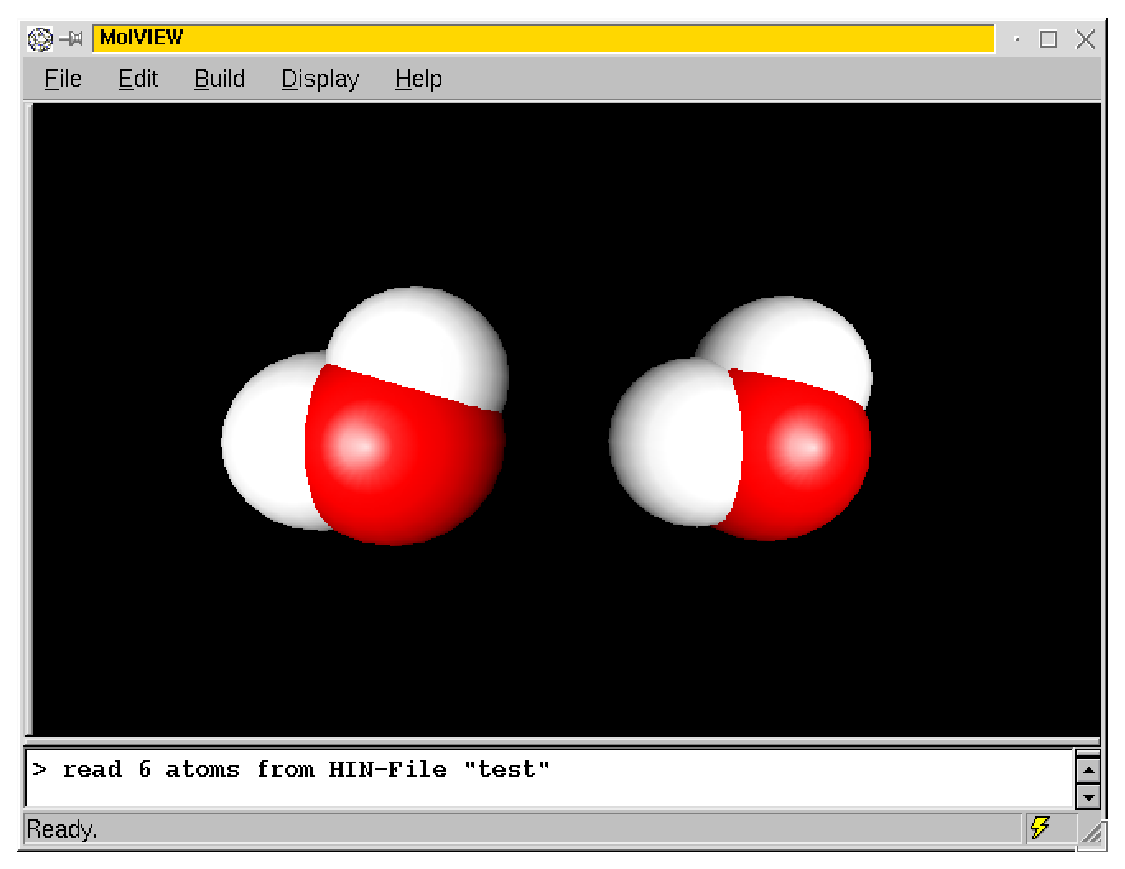
\includegraphics[width=\textwidth]{tut1_screenshot}
	\caption{Screenshot of BALLView showing the result of the first example
					 ({\tt tutorial1.C})}
	\label{fig:tut1-screenshot}
\end{figure}
\noindent
We can now manipulate the two water molecules simultaneously. For example a
further application of the translation processor to the system would apply
the translation to both molecules.
But now we would like to have a look at what we built. So we might write our
system to a file and inspect it with a molecule viewer (\eg BALLView).
BALL supports a variety of file formats. For example we could write the system
to a HyperChem HIN file~\cite{HyperChem}:
\begin{lstlisting}{}
	HINFile outfile("water.hin", File::OUT);
	outfile << S;
	outfile.close();
\end{lstlisting}
\noindent
These three lines of code create a \class{HINFile} object which is used to
read and write HyperChem files. The first line opens a file named {\tt
water.hin} for output ({\tt File::OUT}; if the second argument is omitted the
file is opened for reading only).
The second line uses the stream operator {\tt <<} to write the contents
of system {\tt S} to this file. The file is closed in the third line.

% ????? [anker]
% The following is not true. If we use a pointer here, then it's OK, but
% with a System it simply doesn't work. What do we want here? I'd prefer a
% Sytsem instead of a System*.

% Finally, we have to delete all the objects we created. This is very simple:
% 
% \begin{lstlisting}{}
% 	delete S;
% \end{lstlisting}

\noindent 
As all molecules and atoms we created are inside the system, they are deleted
automatically as soon as the system is deleted.

If this short program is run it creates the following output:

\begin{lstlisting}[frameround=]{}
	# of atoms in water: 3
	# of bonds of oxygen: 2
	# of bonds of hydrogen1: 1
	# of bonds of hydrogen2: 1
	bond distance: 0.95
\end{lstlisting}

\noindent
It also creates a file named {\tt water.hin} which contains the two water
molecules. Fig.~\ref{fig:tut1-screenshot} shows the contents of this file
in the BALLView viewer.

To compile this small example, we still have to include a few header files.
The complete file is shown in Listing~\ref{lst:tutorial1} on
page~\pageref{lst:tutorial1} and can be found in \mbox{{\tt
BALL/source/TUTORIAL/tutorial1.C}}.

First, we have to include \file{iostream} as we use {\tt cout} and {\tt endl}
to print some text. Then, we have to include the headers for the BALL kernel
classes \class{Atom}, \class{Bond}, \class{Molecule}, \class{System}, and
\class{PTE}. The headers for the HyperChem file support are found in the
directory \directory{BALL/FORMAT} and the headers for the
\class{TranslationProcessor} class are found in
{\tt BALL/STRUCTURE/geometricProperties.h}.

As all BALL classes are hidden in the \namespace{BALL} namespace, we have to
give access to this namespace with the command 
\begin{lstlisting}{}
	using namespace BALL;
\end{lstlisting}
Similarly, we also use the namespace \namespace{std} which contains {\tt cout}
and {\tt endl}.

If you have BALL installed, you might now try to compile this example. Simply
change to the directory \directory{BALL/source/TUTORIAL} which contains all
the examples from this tutorial and type 
\begin{lstlisting}[frameround=]{}
	make tutorial1
	./tutorial
\end{lstlisting}
This should build and execute the example. Please remember to set the
environment variable {\tt LD\_LIBRARY\_PATH} to the directory where your
libraries are installed.

After the successful execution of the example, a file named {\tt water.hin}
should appear in the current directory. This file contains the two water
molecules. You might inspect it with the molecule viewer BALLView.
Fig.~\ref{fig:tut1-screenshot} shows a screenshot of BALLView displaying the two
water molecules.

\newpage
\begin{lstlisting}[captionpos=t,caption={The complete source code of the first example.}\label{lst:tutorial1}]{}
// tutorial example 1
// ------------------
// build two water molecules and write them to a file

// needed for cout
#include <iostream>

// the BALL kernel classes
#include <BALL/KERNEL/atom.h>
#include <BALL/KERNEL/bond.h>
#include <BALL/KERNEL/molecule.h>
#include <BALL/KERNEL/system.h>
#include <BALL/KERNEL/PTE.h>

// reading and writing of HyperChem files
#include <BALL/FORMAT/HINFile.h>

// the TranslationProcessor
#include <BALL/STRUCTURE/geometricTransformations.h>

// we use the BALL namespace and the std namespace
using namespace BALL;
using namespace std;

int main()
{
	// we create a new atom called oxygen
	// and set its element to oxygen (PTE[Element::O])
	Atom* oxygen = new Atom;
	oxygen->setElement(PTE[Element::O]);

	// now we create two hydrogen atoms...
	Atom* hydrogen1 = new Atom;
	Atom* hydrogen2 = new Atom;
	hydrogen1->setElement(PTE[Element::H]);
	hydrogen2->setElement(PTE[Element::H]);

	// ...and move them to approximately correct positions
 	hydrogen1->setPosition(Vector3(-0.95, 0.00, 0.0));
 	hydrogen2->setPosition(Vector3( 0.25, 0.87, 0.0));

	// We create our water molecule...
	Molecule* water = new Molecule;

	// ...and insert the three atoms into the molecule.
	water->insert(*oxygen);
	water->insert(*hydrogen1);
	water->insert(*hydrogen2);

	// Then we build the two O-H bonds
	oxygen->createBond(*hydrogen1);
	oxygen->createBond(*hydrogen2);

	// Some statistics: Molecule::countAtoms() 
	// returns the number of atoms, Atom::countBonds() 
	// the number of bonds the atom shares
	cout << "# of atoms in water: " 
			 << water->countAtoms() << endl;
	cout << "# of bonds in oxygen: " 
			 << oxygen->countBonds() << endl;
	cout << "# of bonds of hydrogen1: " 
			 << hydrogen1->countBonds() << endl;
	cout << "# of bonds of hydrogen2: " 
			 << hydrogen2->countBonds() << endl;

	// bond_vector is a vector and is set to the
	// difference of atom positions of oxygen and hydrogen1
	Vector3 bond_vector = oxygen->getPosition() 
											- hydrogen1->getPosition();

	// Vector3::getLength: the length of the vector
	cout << "bond distance: " 
			 << bond_vector.getLength() << endl;

	// Now we copy our molecule using a copy constructor.
	Molecule* water2 = new Molecule(*water);

	// A translation processor moves the second molecule
	// 5 Angstrom along the x axis
	TranslationProcessor translation(Vector3(5, 0, 0));
	water2->apply(translation);

	// We insert our two molecules into a system
	System* S = new System;
	S->insert(*water);
	S->insert(*water2);

	// and write this system to a HyperChem file
	HINFile outfile("water.hin", File::OUT);
	outfile << *S;
	outfile.close();

	// We delete the system. This also deletes 
	// the molecules and the atoms therein
	delete S;
}
\end{lstlisting}

\section{Handling proteins}

In the second example we take a step towards real world applications. Instead
of constructing our own molecules, we now read a protein from a \newterm{PDB
file}. The PDB format~\cite{PDB} is a standardized file format for molecular structure
data. In our case, we will read BPTI (bovine pancreatic trypsin inhibitor), a
small protein:

\begin{lstlisting}{}
	PDBFile infile("bpti.pdb");
	System S;
	infile >> S;
	infile.close();
\end{lstlisting}

\noindent
In the first line, we create a \class{PDBFile} object and assign it to a file
named {\tt bpti.pdb}. Then we create an empty system {\tt S} and read the
contents of the PDB file into the system using the stream operator {\tt >>}.
This use of the stream operators is possible for all file formats in BALL (see
also the first example). Hence, you can easily switch file formats
by changing just the type of the {\tt infile} object (\eg replace it by
\class{HINFile} to read HyperChem files).

We can now verify whether the file was correctly read. BPTI should have 594
atoms. As said before, the number of atoms in any kernel object that might
contain atoms (\ie all classes that are derived from \class{AtomContainer}) is
obtained by calling \method{countAtoms}:

\begin{lstlisting}{}
	cout << "# of atoms in BPTI: " << S.countAtoms() << endl;
\end{lstlisting}

Now, we are interested in the sequence of BPTI. Since BPTI contains only a
single chain, we might just traverse all residues of this chain and write
their names to {\tt cout}. This is done by \newterm{iterators}. Iterators are
objects that can be used to traverse container objects (\eg lists, arrays, or
-- in our case -- proteins). Iterators ``point'' to an element of a container
object. They may be incremented to get the next element and they may be
derferenced similar to pointers by using {\tt *} or {\tt ->}. In fact,
C pointers can be thought of as iterators.
The use of iterators in BALL is similar to the
use of iterators in the \newterm{Standard Template Library} (\Index{STL}).
But there is a significant difference. STL containers usually contain objects of
one single type (\eg a list of strings). In BALL kernel objects, this is
different. A system may contain atoms, proteins, molecules, residues, \etc
This leads to a difference in the interface. A typical {\tt for} loop using STL
iterators to access all elements of a list looks as follows:

\begin{lstlisting}{}
	list<string> string_list = ...;
	list<string>::iterator list_it;
	
	for (list_it = string_list.begin(); 
			 list_it != string_list.end();
			 ++list_it)
	{
		cout << *list_it << endl;
	}
\end{lstlisting}

\noindent
Here, we use a list iterator ({\tt list\_it}) to traverse the whole list ({\tt
string\_list}). The method {\tt begin()} returns an iterator that points to
the first element of the list. In the {\tt for} loop we increment the iterator
until it equals the iterator returned by {\tt end()}. This method returns a
past--the--end iterator, \ie the iterator points beyond the last element of
the container. In the body of the {\tt for} loop, we access the list element
the iterator points to using the {\tt *} operator.

Traversing a BALL kernel data structure is as simple as traversing a list with
STL. But since kernel objects may contain objects of a variety of types,
we have to define over which objects we intend to iterate.
For example iterating over all residues of our system requires a
\class{ResidueIterator}. Clearly, we also need different {\tt begin()} and
{\tt end()} methods for all data types. Hence, the loop that prints the
sequence of our protein reads as follows:

\begin{lstlisting}{}
	ResidueIterator res_it;
	for (res_it = S.beginResidue(); 
			 res_it != S.endResidue();
			 ++res_it)
	{
		cout << res_it->getName() << " ";
	}
	cout << endl;
\end{lstlisting}

\noindent
This loop iterates over all residues in {\tt S} and uses the method {\tt
Residue::}\method{getName()} to access the residues name. All proteins and
residues are traversed in the order in which they appear in the PDB file.
Since the PDB format requires the residues to start with the N-terminus,
the sequence is printed  in the correct order (N-terminus to C-terminus).




\chapter{FAQ}
\label{chapter:faq}
\newpage
\noindent
{\it An up-to-date and searchable version of this FAQ is available at our
website:\\
\FAQURL{http://www.mpi-sb.mpg.de/BALL/}}\\
\hspace{1mm}
\rule{\textwidth}{0.1pt}
\hspace{3mm}
% Max-Planck-Institut f�r Informatik: BALL FAQ
% Point your web browser to: \FAQURL{http://www.mpi-sb.mpg.de/BALL/}
% last generated: Tuesday, April 04, 2000

\FAQCategory{Documentation}
\FAQquestion{Are there Research reports available?}
\FAQanswer{Yes. Publications and research reports on BALL are listed on our website: 
\FAQURL{http://www.bioinf.uni-sb.de/OK/BALL/}
}
\FAQquestion{How do I use BALLView?}
\FAQanswer{There is no documentation available at this time. We are working on it. Just a 
hint: 

Use all three mouse buttons to translate and rotate the objects on the screen
(or mouse button together with SHIFT, ALT, or CTRL, e.g. on Macs).

Shaded menu entries might become available if an adequate number of objects is 
selected (by clicking) in the tree view on the left side of the window.

Some of the functionality is available through context menus accessible
through a right click.

}
\FAQCategory{Installation}
\FAQquestion{Will BALL run on my hardware/with my compiler?}
\FAQanswer{An up-to-date list of all supported platforms can be found on the BALL website 
at 

\FAQURL{http://www.bioinf.uni-sb.de/OK/BALL/Documentation}
}
\FAQCategory{License}
\FAQquestion{Under what kind of license is BALL available?}
\FAQanswer{BALL may be used free of charge for teaching and research. A license for 
commercial use is available upon request from Algorithmic Solutions GmbH (
\FAQURL{http://algorithmic-solutions.com).} 

License terms can be found in the file BALL/source/LICENSE in the source tree.
}



\newpage
\addtocontents{toc}{\protect\contentsline{chapter}{Index}{\thepage}}
\printindex
% the bibliography
%
\renewcommand{\bibname}{References}
\addtocontents{toc}{\protect\contentsline{chapter}{References}{\thepage}}
\bibliographystyle{abbrv}
\bibliography{bib/amber,bib/b_and_cut,bib/BALL,bib/docking,bib/FDPB,bib/tech_rep,bib/software,bib/cpp,bib/computergraphics,bib/chemistry,bib/sw_eng,bib/metrics,bib/BALL.impl,bib/genomics}



\end{document}
